% http://www3.fi.mdp.edu.ar/electrica/medidas1/recursos.html

\chapter{Sobre las mediciones}
\section{Magnitudes}
Medir es \textbf{comparar el valor de una magnitud con otro}, al que se consideró \textbf{la unidad} de dicha magnitud, a través de un experimento físico.

Una \textbf{magnitud} es toda aquella propiedad de un cuerpo que pueda ser medida.

La \textbf{cantidad} es el valor numérico que toma la medida dentro de un sistema de mediciones.

La \textbf{unidad} es la cantidad física que se toma como referencia para hacer las mediciones

\begin{ejemplo}
	Dada la expresión: Altura del edificio = 80 metros,
	\begin{itemize}
		\item Altura es la magnitud.
		\item 80 es la cantidad.
		\item metro es la unidad.
	\end{itemize}
	
	Quiere decir que la altura del edificio (magnitud: longitud) es 80 veces (cantidad) la longitud de referencia denominada metro (unidad).
\end{ejemplo}

Las unidades se fijan según acuerdos internacionales por el Comité Internacional de Pesos y Medidas. Recientemente, en noviembre de 2018, se votó la redefinición de algunas de las unidades fundamentales, incluida el Ampere (para medir corriente eléctrica).

Durante este curso, usaremos el \textbf{Sistema Internacional de Unidades}, pero es posible que en otros contextos se utilicen otros, como el sistema inglés o el CGS.
\subsection{Precisión y exactitud}
	Es común utilizar los términos \textbf{precisión} y \textbf{exactitud} como sinónimos, pero en el ámbito de la metrología, existe una diferencia:
	\begin{itemize}
		\item Precisión se refiere al grado de dispersión del conjunto de valores obtenidos en la medición repetida de una magnitud.
		\item Exactitud se refiere al grado de concordancia entre lo medido y su valor verdadero.
	\end{itemize}
	A su vez, el \textbf{sesgo} es la diferencia entre el valor medido y el valor exacto, que puede ser corregido mediante la calibración. Por lo general, una corrección del sesgo suele mejorar la exactitud, pero no la precisión.
\section{Sistema Internacional de Unidades}
\subsection{Unidades}

\begin{tabular}{|c|c|}
\hline 
Magnitud (símbolo) & Unidad (símbolo) \\ 
\hline 
longitud (L) & metro (m) \\ 
\hline 
masa (M) & kilogramo (kg) \\ 
\hline 
tiempo (T) & segundo (s) \\ 
\hline 
corriente eléctrica (I) & ampere (A) \\ 
\hline 
temperatura ($ \Theta $) & kelvin (K) \\ 
\hline 
intensidad lumínica (J) & candela (cd) \\ 
\hline 
energía (E) & julio (J) \\ 
\hline 
fuerza (F) & newton (N) \\ 
\hline 
potencia (P) & vatio (W) \\ 
\hline 
carga eléctrica (Q) & coulomb (C) \\ 
\hline 
tensión eléctrica, diferencia de potencial (V) & voltio (V) \\ 
\hline 
capacitancia & faradio (F) \\ 
\hline 
resistencia eléctrica (R) & ohmio ($ \Omega $) \\ 
\hline 
flujo magnético & weber (Wb) \\ 
\hline 
campo magnético & tesla (T) \\ 
\hline 
inductancia (L) & henrio (H) \\ 
\hline 
flujo luminoso & lumen (lm) \\ 
\hline
frecuencia & hertz (Hz) \\ 
\hline
\end{tabular} 

\subsection{Prefijos}\label{section:prefijos}

\begin{tabular}{|c|c|c|}
\hline 
Factor de multiplicación & Nombre  & Sı́mbolo  \\
\hline 
$10^{24}$                    & yotta   & Y       \\
$10 ^{21}$                    & zetta   & Z       \\
$10 ^{18}$                    & exa     & E       \\
$10 ^{15}$                    & peta    & P       \\
$10 ^{12}$                    & tera    & T       \\
$10 ^{9}$                     & giga    & G       \\
$10 ^{6}$                     & mega    & M       \\
$10 ^{3}$                     & kilo    & k       \\
$10 ^{2}$                     & hecto ∗ & h       \\
$10 ^{1}$                     & deka ∗  & da      \\
$10 ^{-1}$                    & deci ∗  & d       \\
$10 ^{-2}$                    & centi ∗ & c       \\
$10 ^{-3}$                    & mili    & m       \\
$10 ^{-6}$                    & micro   & $\mu $       \\
$10 ^{-9}$                    & nano    & n       \\
$10 ^{-12}$                   & pico    & p       \\
$10 ^{-15}$                   & femto   & f       \\
$10 ^{-18}$                   & atto    & a       \\
$10 ^{-21}$                   & zepto   & z       \\
$10 ^{-24}$                   & yocto   & y \\ \hline 
\end{tabular}

\subsection{Reglas}
\begin{enumerate}
	\item Los símbolos son siempre impresos en letra tipo romana, indistintamente del tipo de letra usado en el resto del texto.
	\item Los símbolos son escritos en minúscula excepto cuando el nombre de la unidad se deriva de un nombre propio.
	\item Los símbolos de los prefijos se imprimen en letra tipo romana sin espacio entre los sı́mbolos del prefijo y la unidad.
	\item Los símbolos nunca se pluralizan.
	\item Nunca use un punto después de un sı́mbolo, excepto cuando el sı́mbolo ocurre al final de una oración.
	\item Siempre use un espacio entre el número y el sı́mbolo, excepto cuando el primer caracter de un símbolo no es una letra.
	\item Los símbolos se usan en conjunto con números en lugar de escribir el nombre completo de la unidad; cuando no hay números, las unidades se escriben con su nombre propio.
	
\end{enumerate}
\section{Consideraciones para la lectura de mediciones}
\subsection{Cifras significativas}
Según el nivel de precisión que se requiera en una medición, será necesario utilizar una determinada cantidad de cifras significativas.

Existen magnitudes continuas, que son aquellas que entre dos valores poseen infinitas posibilidades, y magnitudes discretas, que entre dos valores cualesquiera poseen una cantidad numerable y finita de posibilidades.

\begin{ejemplo}
	\begin{itemize}
		\item La cantidad de conductores dentro de una caja es una magnitud discreta (puede haber uno, dos, diez o incluso ningún cable, pero no 1,3 cables).
		\item La longitud de un conductor es una magnitud continua (puede medir 0,5 m, o 0,554 m, o 0,5533223 m).
	\end{itemize}
\end{ejemplo}

Las mediciones de magnitudes continuas siempre serán aproximadas, y las mediciones de magnitudes discretas, en muchos casos, pueden ser exactas.

El número de cifras significativas determinan la precisión de una medición.

Siempre que se opere con dos medidas, la precisión de ambas deberá ser consistente. Esto significa que si se suma una medición con precisión de decimales con otra con precisión de milésimos, el resultado será impreciso. En estos casos, el número con menor precisión determinará la precisión de la solución.
\subsection{Redondeo}
En muchos casos, será necesario redondear las mediciones. Para ello, se toma la lectura hasta el último dígito significativo que se esté considerando, sumando 1 al mismo si el próximo dígito es mayor o igual que 5, o dejándolo como está (truncar) si el próximo dígito es menor que 5.

\begin{ejemplo}
Si $V_1=3,25 V$, $V_2=2,4201 V$ y $V_3=3,245V$, 
	\begin{itemize}
		\item $V_1+V_2=3,25 V + 2,4201 V=5,6501 V=5,65 V$
		\item $V_1+V_3=3,25 V + 3,245 V = 6,495 V $. Como el número con menor precisión tiene dos dígitos decimales, deberá redondearse, sumando una unidad a las centésimas (porque el dígito de las milésimas es 5) obteniendo $6,50 V$ o $6,5V$.
	\end{itemize}
\end{ejemplo}
\subsection{Notación científica y de ingeniería}
En la sección \ref{section:prefijos}, se han usado, como factores de multiplicación, potencias de 10.

A veces, cuando los valores con los que se trabaja son muy grandes o muy pequeños, suele ser cómodo utilizar potencias de 10. De ese modo, puede expresarse estos valores indicando sólo sus cifras significativas, multiplicadas por una potencia de 10.

Si la potencia es positiva, el factor de multiplicación será un 1 y tantos ceros como indique el exponente:

\begin{tabular}{|c|c|c|}
\hline 
Valor & Potencia & Operación \\ 
\hline 
$1$ & $10^0$ & $10/10$ \\ 
\hline 
$10$ & $10^1$ & $10$ \\ 
\hline 
$100$ & $10^2$ & $10 \times 10$ \\ 
\hline 
$1000$ & $10^3$ & $10 \times 10 \times 10$ \\ 
\hline 
... & ... & ... \\ 
\hline 
1 y $n$ ceros & $10^n$ & $10 \times 10 \times 10 ... n$ veces \\ 
\hline 
\end{tabular} 

Si la potencia es negativa, debe recordarse la siguiente propiedad de las potencias:

$$ \frac{1}{10^{n}}=10^{-n} $$

Esto da lugar al siguiente razonamiento:

\begin{tabular}{|c|c|c|}
\hline 
Valor & Potencia & Operación \\ 
\hline 
$0,1$ & $10^{-1}$ & $1/10$ \\ 
\hline 
$0,01$ & $10^{-2}$ & $1/100$ \\ 
\hline 
$0,001$ & $10^{-3}$ & $1/1000$ \\ 
\hline 
$0,0001$ & $10^{-4}$ & $1/10000$ \\ 
\hline 
... & ... & ... \\ 
\hline 
$0,(n-1)$ ceros y $1$ & $10^{-n}$ & $1/1(n$ ceros $)$ \\ 
\hline 
\end{tabular}

\begin{ejemplo}
Expresar los siguientes valores en forma decimal.
	\begin{itemize}
		\item $ 3 \times 10^{-3}=3\times \frac{1}{1000}=3\times 0,001 = 0,003 $
		\item $ 12 \times 10^{4}= 12 \times 1000 = 12000 $
		\item $ 3,25 \times 10^{6} = 3,25 \times 1000000 = 3250000 $
		\item $ 3,25 \times 10^{-4}= 3,25 \times 0,0001 = 0,000325 $
	\end{itemize}
\end{ejemplo}

En los ejemplos anteriores, se procedió a multiplicar un número por una potencia de 10, para obtener valores más pequeños o más grandes, y a simple vista resulta más legible.

Es una convención en notación científica, que la mantisa o coeficiente por el cual se multiplique la potencia de 10, debe estar entre 1 y 10.

La notación de ingeniería es similar, excepto que los exponentes de la potencia de 10 deben ser múltiplos de 3 y la mantisa debe estar entre 1 y 1000. Esto permite utilizar prefijos de magnitud como los que se enunciaron en la sección \ref{section:prefijos}.

\begin{ejemplo}
	\begin{itemize}
	Convertir las siguientes medidas para eliminar los prefijos, según la tabla de la sección \ref{section:prefijos}.
		\item $ 3 \mu F = 3\times 10^{-6} F=0,000003 F$
		\item $ 1,2 mA = 1,2 \times 10^{-3} A= 0,0012 A$
		\item $ 120 pF = 120 \times 10^{-12} F=0,000000000120 F$
		\item $ 22 M\Omega = 22 \times 10^{6} \Omega = 22000000 \Omega $
	\end{itemize}
\end{ejemplo}

\section{Mediciones directas e indirectas}

Una medición directa es la que se realiza con un instrumento sobre un determinado elemento, mientras que una medición indirecta involucrará, además, algún paso adicional mediante el cálculo.
\begin{ejemplo}
	
	\begin{itemize}
	
		\item Medir la tensión de un tomacorriente con un voltímetro es una medición directa.
		\item Con un voltímetro se mide la tensión en una rama de un circuito de CC. Luego se mide la corriente con un amperímetro en serie. Finalmente, se multiplican ambos resultados y con ello se obtiene la medición indirecta de la potencia.
	\end{itemize}		
\end{ejemplo}

\section{Generalidades de instrumentos de medición eléctrica}

\subsection{Instrumentos analógicos}

\begin{figure}[htbp]
  \centering
  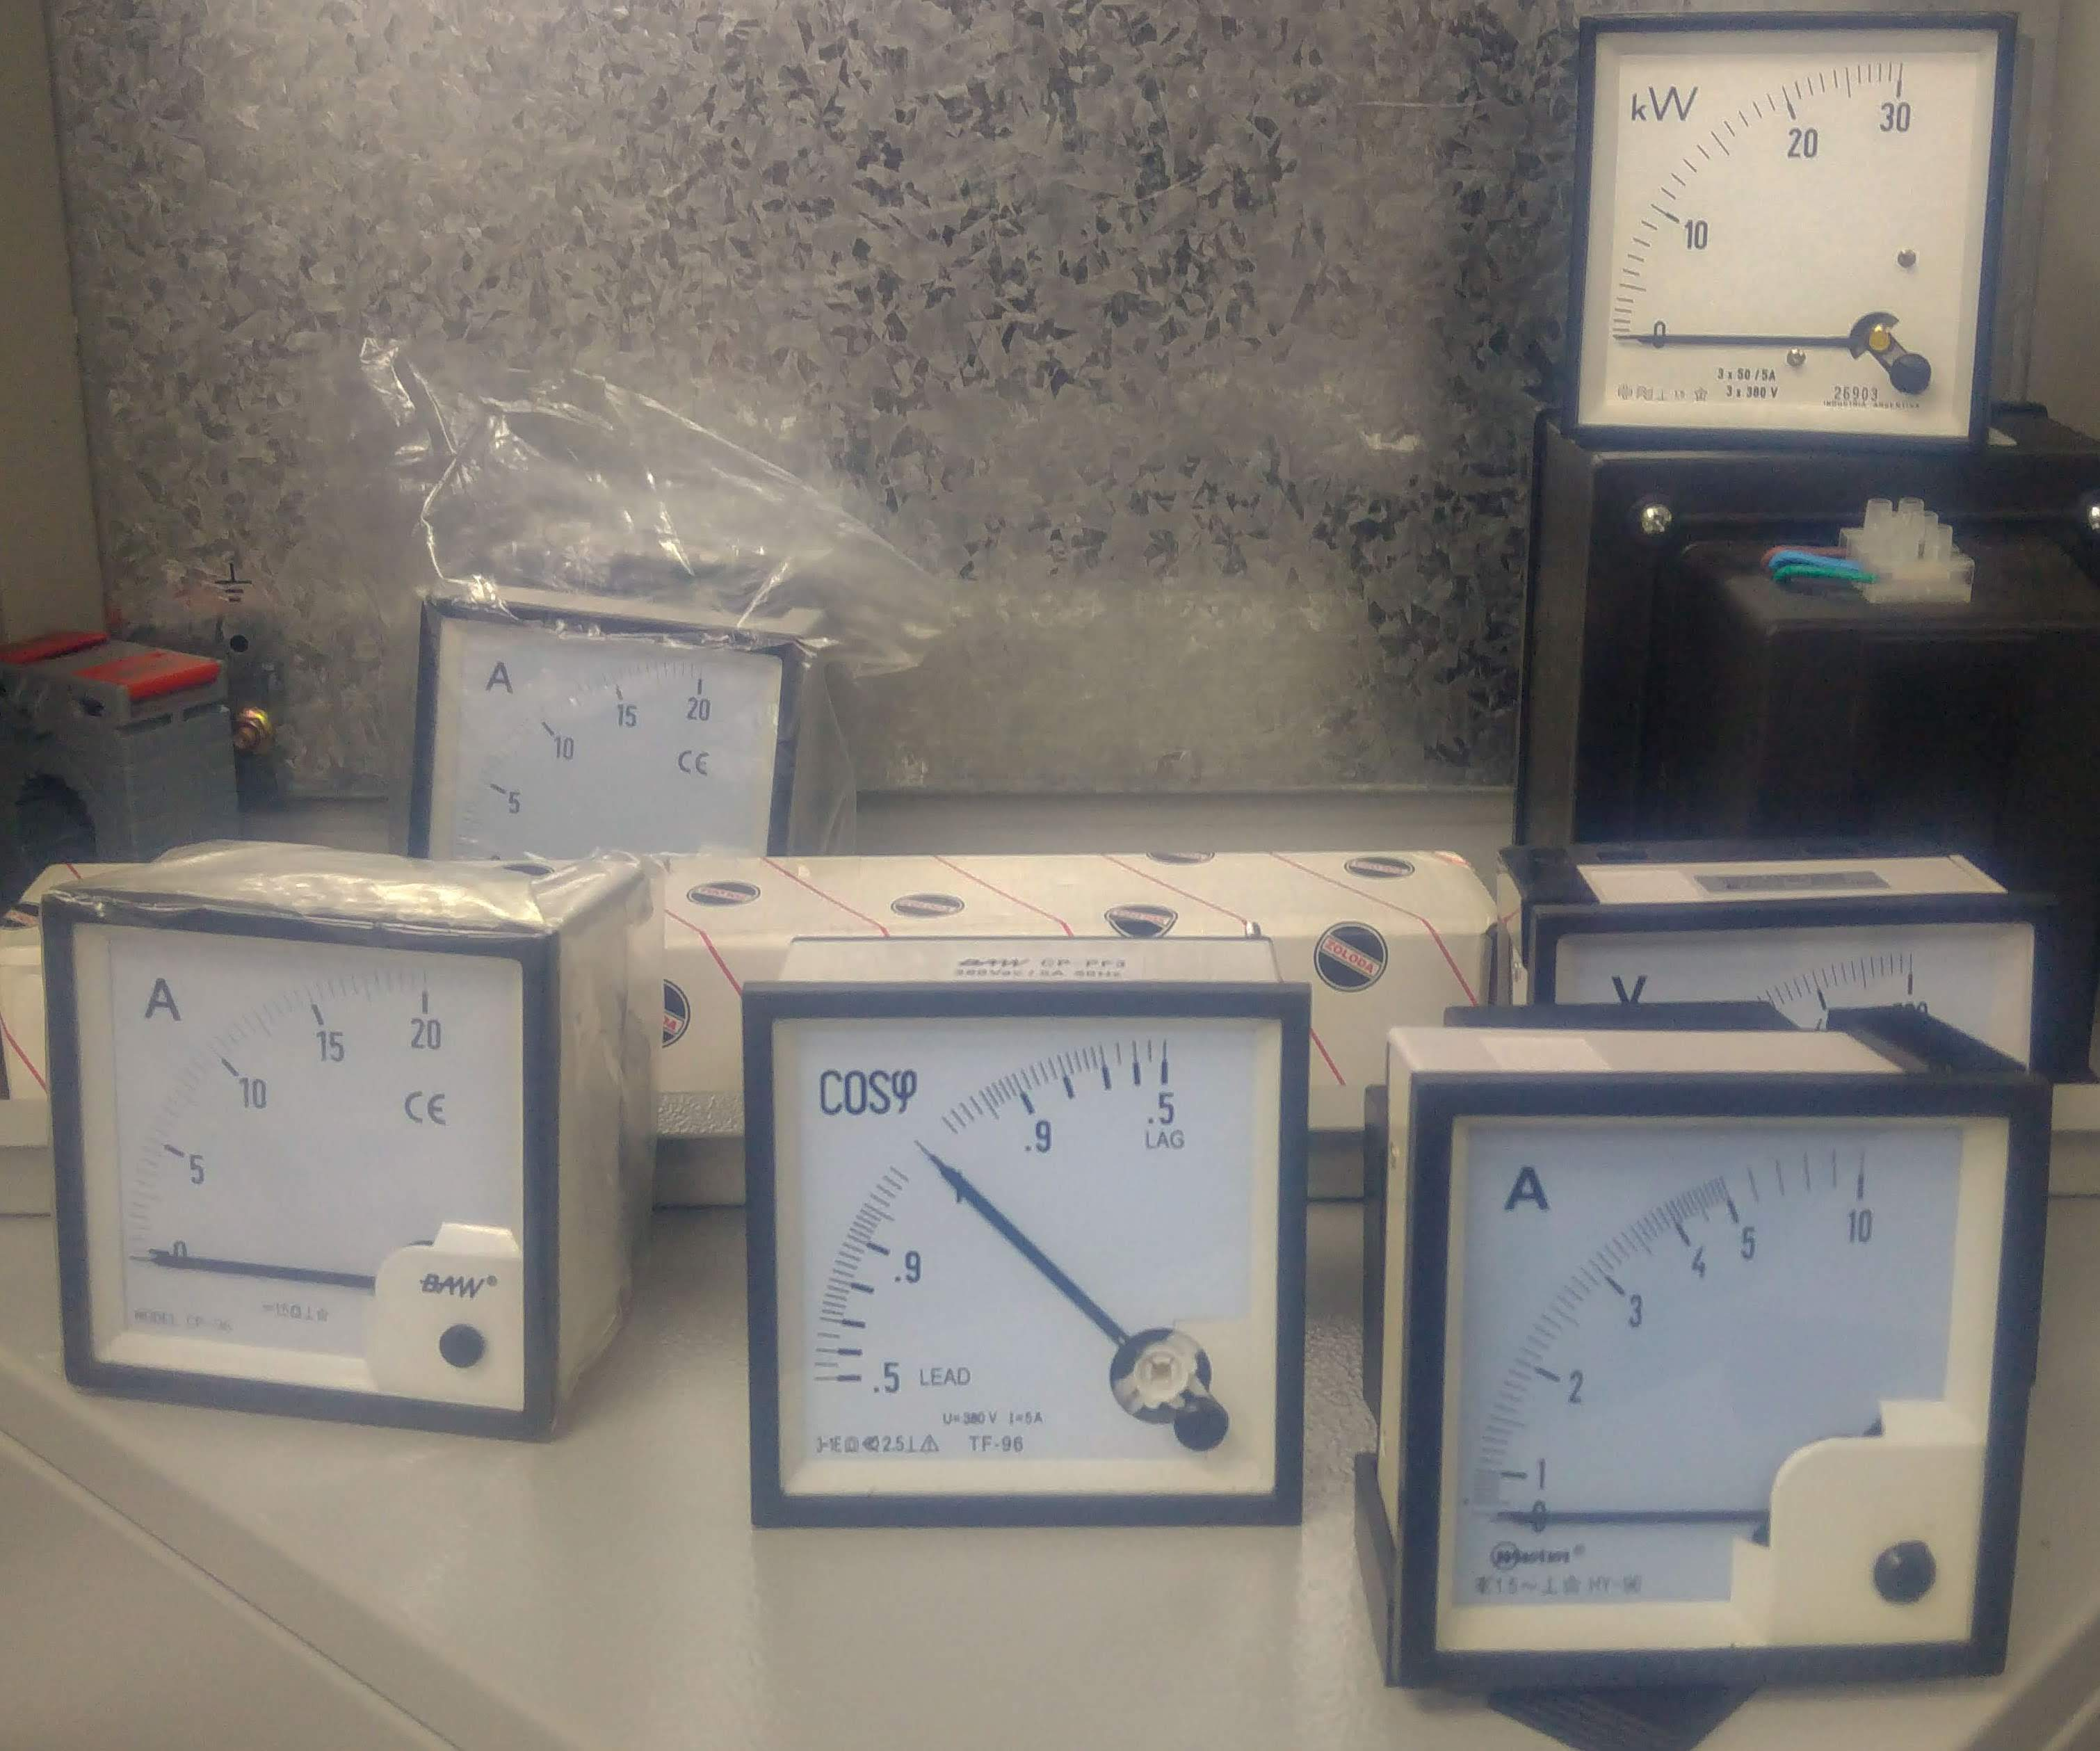
\includegraphics[width=\textwidth,height=\textheight,keepaspectratio]{images/fotos/analogicos.jpg}
  \caption{Instrumentos analógicos de medición de magnitudes eléctricas}
  \label{fig:instrumentos_analogicos}
\end{figure}

Los instrumentos de medición analógicos utilizan una aguja para visualizar las lecturas mediante una aguja, que se mueve de manera continua, al igual que la magnitud que se intenta medir.

En muchos casos, no requieren de alimentación externa, se visualiza de forma más sencilla la variación (crecimiento o decrecimiento) y no son muy sofisticados. 

Por otra parte, son más tendenciosos a errores de lectura groseros (por las confusiones en cuanto a las escalas), y tienen poca resolución.

Los instrumentos de medición analógica poseen un \textbf{alcance}, que es el valor máximo que puede medir dicho instrumento y una cantidad de divisiones denominadas \textbf{deflexiones}, que serán las que indiquen el valor medido según la posición de la aguja.

A partir de estas medidas, puede calcularse la \textbf{constante de lectura K}, que es la relación entre el alcance y la máxima cantidad de deflexiones. Esta medida indica la mínima unidad de variación legible.
$$ K = \frac{Alcance}{\alpha MAX} $$

El \textbf{rango de medida} es el tramo de la escala en el cual las lecturas son confiables mientras que el \textbf{rango de indicación} corresponde a toda la escala del instrumento.

\subsection{Instrumentos digitales}
	
Los instrumentos digitales muestran un número de varias cifras en vez de una escala continua. Lo hacen mediante un display digital de varios dígitos, y a veces con alertas sonoras o lumínicas.

Si bien su construcción es más compleja que la de los instrumentos analógicos y requieren una alimentación externa en todos los casos, tienen una alta resolución, evitan los errores de lectura, modifican muy poco el circuito en el que se conectan (impedancia de entrada muy alta) y son muy rápidos.

En algunos casos, se incluye la selección automática de escalas y permiten introducir sus datos directamente en otro sistema (computadoras) para poder procesarlos.

Los instrumentos digitales poseen una determinada \textbf{cantidad de dígitos}, que pueden ir de 0 a 9 y un \textbf{dígito de sobrerrango}, que sólo puede mostrar 0 ó 1.

La \textbf{sensibilidad}, en un instrumento digital, corresponde a el dígito menos significativo del rango.

La \textbf{resolución}, por otra parte, no tiene unidad. Para calcularla, se debe pensar en la máxima lectura posible y dividir el valor mínimo que puede medir el último dígito sobre esta lectura máxima. Esto quiere decir, que es el menor cambio posible a observar en la cantidad medida. 

$$ \textit{Resolución} = \frac{1}{10^{d}} \textit{siendo $d$ la cantidad de dígitos}$$

La resolución también se suele expresar como porcentaje.

Con estos datos, se puede hallar la sensibilidad en función de la resolución del instrumento:
$$ \text{Sensibilidad} = \frac{\textit{Resolución x Valor a plena escala}}{1000} $$

La \textbf{deriva de la sensibilidad} es la variación que sufre la sensibilidad como consecuencia de las condiciones ambientales en las que se realiza el experimento de medición.

\subsection{Clase de un instrumento}
La clase de un instrumento es uno de los indicadores de la precisión del mismo. Es el valor porcentual que expresa la relación entre el error absoluto y el alcance del mismo:

$$ Clase = \frac{E_{abs}max}{Alcance}\times 100 $$
\begin{figure}
	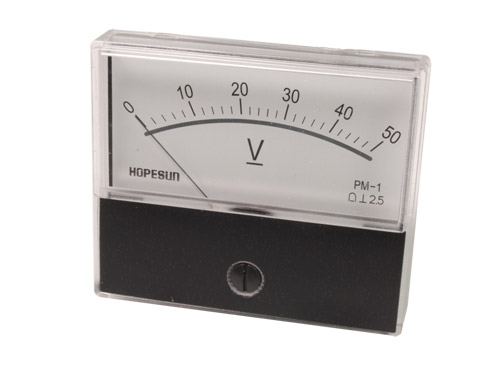
\includegraphics[scale=0.7]{images/volt_clase}
	\caption{Voltímetro Clase 2,5}
	\label{fig:voltclase}
\end{figure}
\begin{ejemplo}
	En la figura \ref{fig:voltclase}, se puede apreciar que la clase del instrumento es 2,5. Como se ve, el alcance máximo es de 50 V. ¿Cuál es el error absoluto máximo que puede producirse?
	
	\emph{Solución:} Reemplazando en la ecuación de clase:
	
	$$ 2,5 = \frac{ErrorAbsMax}{50 V} \times 100 
	\rightarrow
	ErrorAbsMax = \frac{2,5 \times 50V}{100} = 1,25 V $$
	
	
\end{ejemplo}

\begin{tabular}{|c|p{7cm}|}
\hline 
Clase del instrumento & Aplicación \\ 
\hline 
0.05 a 0.1 & Patrones de referencia. Calibración de instrumentos. Ensayos de laboratorio muy precisos. \\ 
\hline 
0.2 a 0.5 & Ensayos de laboratorio. Contraste de instrumentos de una clase al menos 5 veces mayor \\ 
\hline 
>1 & Tableros, paneles de escala vertical, instrumentos portátiles de baja precisión. \\ 
\hline 
\end{tabular} 

\subsection{Simbología de los instrumentos de medición eléctrica}
